% Introduction
\chapter{Introduction}\label{introduction}
	Route planning refers to the problem of finding an \textit{optimal} route between given locations in a network.
	With the ongoing expansion of road and public transit networks all over the world route planner gain more and
	more importance. This led to a rapid increase in research \libref{routePlanningOverview, networks, transitModels}
	of relevant topics and development of route planner software \libref{navHistoryEarly, navHistoryNewer, vehicleNavigation}.\\\\
	However, a common problem of most such services is that they are limited to one transportation mode only.
	That is a route can only be taken by a car or train, but not with both at the same time. This is known as \uniModal routing.
	In contrast to that \multiModal routing allows the alternation of transportation modes. For example a route that
	first uses a car to drive to a train station, then a train which travels to a another train station and finally
	using a bicycle from there to reach the destination.
	
	The difficulty with \multiModal routing lies in most algorithms being fitted to networks with specific properties.
	Unfortunately, road networks differ a lot from public transit networks. As such, a route planning algorithm
	fitted to a certain type of network will likely yield undesired results, have an impractical running time or not
	even be able to be used at all on different networks. We will explore this later in \sectionref{evaluation}.

% Related Work
\section{Related Work}
	Research on route planning began roughly in the \datef{1950}s with the development of \dijkstra \libref{dijkstra} and the
	\bellmanFord \libref{dijkstra}. Ten years later \dijkstra was improved using certain heuristics, introducing \astar \libref{alt}.
	While these algorithms are all able to compute the shortest path in a road network, they are too slow on real world networks of
	realistic size, such as the scale of a country or even a state.
	
	Thus, starting from \datef{2000}, research focused on developing speedup techniques for \dijkstra. Basic techniques include
	bi-directional search, goal-directed search and contraction. In \datef{2005} \astar was further
	improved by introducing a heuristic based on \textit{landmarks}, exploiting properties of the triangle inequality,
	called \alt \libref{alt}. Around the same time, techniques based on edge labels were developed. A prominent refinement of this
	approach is called \arcFlags \libref{arcFlags}. In \datef{2008}, contraction hierarchies (\ch) \libref{ch} was presented as a
	very efficient algorithm based on contraction. Also, transit node routing (\tnr) \libref{tnr}, a technique based on \textit{access nodes},
	was developed. A year later, it was shown that approaches can efficiently be combined, yielding very fast solutions.
	Resulting in \chase \libref{chase}, which combines \ch with \arcFlags, and a combination of \tnr and \arcFlags, that yield query times
	of around $0.005$ milliseconds on road networks of country size (compare to \figref{uniModalTimeIndependentResultsExternalOverview}
	in \sectionref{evaluation}).\\\\
	For public transportation networks, research was first focused on adapting existing solutions for road networks.
	From \datef{2005} to \datef{2012} most of the mentioned algorithms were successfully extended to compute shortest
	paths in public transportation networks \libref{networks, simpleTimeExpanded, transitModels, tnrTransit, routePlanningOverview}.
	Unfortunately, most do not perform well on transit networks, as such networks have a completely different structure from which
	previous speedup techniques do not benefit much.
	
	Because of that, techniques designed especially for transit networks have been developed. Efficient algorithms include \transferPatterns
	\libref{transferPatterns} from \datef{2010}, \raptor \libref{raptor} from \datef{2012} and \csa \libref{csa} from \datef{2017}.\\\\
	A similar approach was done for \multiModal routing, where most algorithms have been adapted to also run in combined networks,
	accounting for transportation mode restrictions \libref{labelShortestPath, alt, lcsppShortcuts}.
	However, the topic is still relatively new and promising approaches, as well as extensive research, appear only since around
	\datef{2008}. Theoretical background was provided by \libref{labelShortestPath, lcssp}.
	Nowadays, research is focused on \anr \libref{accessNodeRouting, routePlanningOverview}, a general approach for combining
	multiple networks using \text{access nodes}. As well as on improving techniques for solving related subproblems, such as
	efficient access node selection and solving the \lcspp \libref{labelShortestPath} with less restrictions.\\\\
	Meanwhile, related, more practice-oriented problems are studied, such as penalizing turns \libref{turnPenaltiesOld, turnPenaltiesNew}
	or general multi criteria routing \libref{multiCriteria, multiCriteriaSelection, routePlanningOverview}.

% Contributions
\section{Contributions}
	Our main contribution to this research field is the development of \cobweb \libref{cobweb}, which is an open-source
	framework for \multiModal route planning developed in the context of this thesis. Further, in \sectionref{evaluation}
	we give a detailed evaluation of experiments demonstrating the effectiveness of our implementations for all algorithms
	explained in this thesis. Additionally, we give an overview over route planning and relevant approaches, as well as a
	thorough explanation for all used algorithms including examples illustrating them.\\\\
	\cobweb is able to parse networks given in the \osm and \gtfs format, which we will explore later in \sectionref{inputData_sec}, as well as
	in compressed formats, such as \bzipTwo \libref{bzipTwoFormat}, \gzip \libref{gzipFormat}, \zip \libref{zipFormat} and \xz \libref{xzFormat}.
	Networks are then represented in one of the models presented in \sectionref{models}. Metadata, like names of roads, are saved in an external
	database and retrieved again later.\\\\
	The back end offers three {\restApi}s \libref{rest} using a client-server-based structure communicating over the \http \libref{http} which
	are written primarily in \java.
	One \api is for planning journeys, one for searching nodes by their name and one for retrieving the nearest node to a given location.
	
	The routing \api answers journey planning requests from a given source to a destination. The answer contains multiple viable journeys.
	A request consists of
	\begin{itemize}
		\item[1.] \depTime, the departure time to start journeys at;
		\item[2.] \modes, transportation modes allowed for the journey. Applicable are \car, \bike, \foot and \tram;
		\item[3.] \fromJ, the source node to depart from;
		\item[4.] \toJ, the destination node to travel to.
	\end{itemize}
	The server then computes journeys using the algorithms presented in \sectionref{shortestPathProblem} and responds with a list of viable
	journeys. A journey mainly consists of geographical coordinates describing the path to travel along and metadata, such as which
	transportation mode to use for which segment, names of roads and time information for each segment.
	
	The name search \api finds \osm nodes by their name. Therefore, we developed \lexiSearch \libref{lexiSearch}, an \api for retrieving
	information from given datasets.
	It maintains the names of \osm nodes in an inverted $n$-gram index \libref{nGram, invertedIndex}. This makes it possible to efficiently
	retrieve nodes by an approximate name which is allowed to have errors, such as spelling mistakes. This is known as fuzzy search, or
	approximate string matching, see \libref{fuzzySearch} for details. Further, nodes can be retrieved by prefixes, yielding search
	results \textit{as-you-type}. For example, a request with the approximate prefix name \textit{Freirb} would yield nodes with
	the name \textit{Freiburg} and \textit{Freiburg im Breisgau}.
	
	The third \api offers retrieval of the \osm node nearest to a given geographical coordinate. Making it possible for a client to plan a
	route from an arbitrary location to an arbitrary destination, for example by clicking on a map. \cobweb retrieves the nearest node by
	using a \coverTree and solving the \nearestNeighborProblem, as explained in \sectionref{nearestNeighborProblem}.\\\\
	% Cobweb front end screenshot
	\begin{figure}[!ht]
		 \begin{center}
			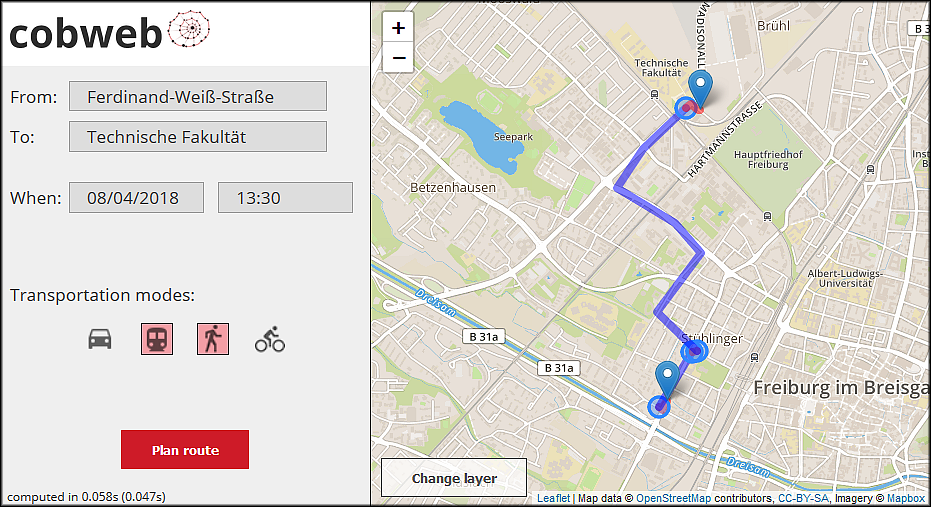
\includegraphics[scale=0.5]{res/cobweb_frontend}
		\end{center}
		\caption{Screenshot of {\cobweb}s \libref{cobweb} front end, an open-source \multiModal route planner. It shows a \multiModal
		route starting from a given source, using the modes \textit{foot-tram-foot-tram-foot} in that sequence to reach the destination.}
		\label{cobweb_frontend}
	\end{figure}\quad\\
	\cobweb comes with a light web-based front end (see \figref{cobweb_frontend} for an image). Its interface is very similar to other
	route planning applications, providing input fields for a source and a destination, as well as a departure time and transportation mode
	restrictions. The front end is primarily written in \js and communicates with the back ends {\restApi}s using asynchronous method invocations.
	The resulting journeys are displayed on a map and highlighted according to metadata, such as the used transportation mode.\\\\
	The source code of \cobweb, a release candidate, as well as a detailed description of the project, its {\api}s, an installation guide,
	the structure and its control flow, can be found at \libref{cobweb}.
	
% Overview
\section{Overview}
	In this thesis, we explore a technique with which we can combine an algorithm fitted for road networks with an algorithm
	for public transit networks. Effectively obtaining a generic algorithm that is able to compute routes on combined networks.
	The basic idea is simple, given a source and destination, both in the road network, we select \textit{access nodes} for both.
	These are nodes where we will switch from the road into the public transit network. A route can then be computed by
	using the road algorithm for the source to its access nodes, the transit algorithm for the access nodes of the source
	to the access nodes of the destination and finally the road algorithm again for the destinations access nodes to
	the destination. Note that this technique might not yield the shortest possible path anymore. Also, it does not allow
	an arbitrary alternation of transportation modes. However, we accept those limitations since the resulting
	algorithm is very generic and able to compute routes faster than without limitations. We will cover this technique in detail
	in \sectionref{accessNodes}.\\\\
	Our final technique uses a modified version of \alt \libref{alt} as road algorithm and \csa \libref{csa} for the transportation network.
	The algorithms are presented in \sectionref{alt} and \sectionref{csa} respectively.
	We also develop a \multiModal variant of \dijkstra \libref{dijkstra}, which is able to compute the shortest route in a combined
	network with the possibility of changing transportation modes arbitrarily. It is presented in \sectionref{modifiedDijkstra}
	and acts as a baseline to our final technique based on access nodes.
	
	We compute access nodes by solving the \nearestNeighborProblem. For a given node in the road network its access
	nodes are then all nodes in the transit network, which are in the \textit{vicinity} of the road node. We explore a solution
	to this problem in \sectionref{nearestNeighborProblem}.\\\\
	\sectionref{models} starts by defining types of networks. We represent road networks by graphs only.
	For transit networks, we provide a graph representation too. Both graphs can then be combined into a linked graph.
	The advantage of graph based models is that they are well studied and therefore we are able to use our
	\multiModal variant of \dijkstra to compute routes on them.
	However, we also propose a non-graph based representation for transit networks, a timetable. The timetable is used by \csa,
	an efficient algorithm for route planning on public transit networks. With that, our road and transit networks get incompatible
	and can not easily be combined. Therefore, we use the previously mentioned generic approach based on access nodes
	for this type of network.\\\\
	Further, we implemented the presented algorithms in the \cobweb \libref{cobweb} project, which is an open-source \multiModal
	route planner. In \sectionref{evaluation} we show our experimental results and compare the techniques with each other.